\documentclass[referat]{SCWorks}
% Тип обучения (одно из значений):
%    bachelor   - бакалавриат (по умолчанию)
%    spec       - специальность
%    master     - магистратура
% Форма обучения (одно из значений):
%    och        - очное (по умолчанию)
%    zaoch      - заочное
% Тип работы (одно из значений):
%    coursework - курсовая работа (по умолчанию)
%    referat    - реферат
%  * otchet     - универсальный отчет
%  * nirjournal - журнал НИР
%  * digital    - итоговая работа для цифровой кафдры
%    diploma    - дипломная работа
%    pract      - отчет о научно-исследовательской работе
%    autoref    - автореферат выпускной работы
%    assignment - задание на выпускную квалификационную работу
%    review     - отзыв руководителя
%    critique   - рецензия на выпускную работу
% Включение шрифта
%    times      - включение шрифта Times New Roman (если установлен)
%                 по умолчанию выключен
\usepackage{preamble}

\begin{document}

% Кафедра (в родительном падеже)
\chair{математической кибернетики и компьютерных наук}

% Тема работы
\title{Специалист по защите информации}

% Курс
\course{1}

% Группа
\group{111}

% Факультет (в родительном падеже) (по умолчанию "факультета КНиИТ")
% \department{факультета КНиИТ}

% Специальность/направление код - наименование
 \napravlenie{02.03.02 "--- Фундаментальная информатика и информационные технологии}
% \napravlenie{02.03.01 "--- Математическое обеспечение и администрирование информационных систем}
% \napravlenie{09.03.01 "--- Информатика и вычислительная техника}
%\napravlenie{09.03.04 "--- Программная инженерия}
% \napravlenie{10.05.01 "--- Компьютерная безопасность}

% Для студентки. Для работы студента следующая команда не нужна.
\studenttitle{Студентов}

% Фамилия, имя, отчество в родительном падеже
\author{Коновалова Александра Сергеевича, Пицика Харитона Николаевича}

% Заведующий кафедрой 
\chtitle{доцент, к.\,ф.-м.\,н.}
\chname{С.\,В.\,Миронов}

% Руководитель ДПП ПП для цифровой кафедры (перекрывает заведующего кафедры)
% \chpretitle{
%     заведующий кафедрой математических основ информатики и олимпиадного\\
%     программирования на базе МАОУ <<Ф"=Т лицей №1>>
% }
% \chtitle{г. Саратов, к.\,ф.-м.\,н., доцент}
% \chname{Кондратова\, Ю.\,Н.}

% Научный руководитель (для реферата преподаватель проверяющий работу)
\satitle{доцент, к.\,п.\,н.} %должность, степень, звание
\saname{А.\,П.\,Грецова}

% Руководитель практики от организации (руководитель для цифровой кафедры)
\patitle{доцент, к.\,ф.-м.\,н.}
\paname{С.\,В.\,Миронов}

% Руководитель НИР
\nirtitle{доцент, к.\,п.\,н.} % степень, звание
\nirname{В.\,А.\,Векслер}

% Семестр (только для практики, для остальных типов работ не используется)
\term{2}

% Наименование практики (только для практики, для остальных типов работ не
% используется)
\practtype{учебная}

% Продолжительность практики (количество недель) (только для практики, для
% остальных типов работ не используется)
\duration{2}

% Даты начала и окончания практики (только для практики, для остальных типов
% работ не используется)
\practStart{01.07.2022}
\practFinish{13.01.2023}

% Год выполнения отчета
\date{2024}

\maketitle

% Включение нумерации рисунков, формул и таблиц по разделам (по умолчанию -
% нумерация сквозная) (допускается оба вида нумерации)
\secNumbering

\tableofcontents

% Раздел "Обозначения и сокращения". Может отсутствовать в работе
% \abbreviations
% \begin{description}
%     \item ... "--- ...
%     \item ... "--- ...
% \end{description}

% Раздел "Определения". Может отсутствовать в работе
% \definitions

% Раздел "Определения, обозначения и сокращения". Может отсутствовать в работе.
% Если присутствует, то заменяет собой разделы "Обозначения и сокращения" и
% "Определения"
% \defabbr

\intro

% После введения — серии \section, \subsection и т.д.
\section{Понятие защиты информации.}
\subsection{Общее представление о защите информации.}
Современные методы обработки, передачи и накопления информации с помощью информационный систем способствовали 
появлению угроз, связанных с возможностью потери, искажения и раскрытия данных, адресованных или принадлежащих 
конечным пользователям. Поэтому обеспечение информационной безопасности компьютерных систем и сетей становится 
одним из основных направлений в области информационных технологий\cite{sh}.

Словосочетание «информационная безопасность» в разных контекстах может иметь различный смысл. В Доктрине информационной
безопасности Российской Федерации термин «информационная безопасность» используется в глобальном смысле. Имеется в виду 
состояние защищенности национальных интересов в информационной сфере, определяемых совокупностью сбалансированных интересов 
личности, общества и государства. 

Под информационной безопасностью в узком смысле стоит понимать защищенность информации и поддерживающей инфраструктуры от 
случайных или преднамеренных воздействий естественного или искусственного характера, которые могут нанести неприемлемый ущерб 
субъектам информационных отношений, в том числе владельцам и пользователям информации и поддерживающей инфраструктуры. 

Таким образом, \textbf{защита информации} "---  это совокупность действий, направленных на обеспечение информационной безопасности\cite{untuit}.

Можно выделить несколько основных задач, решение которых в информационных системах и телекоммуникационных сетях обеспечивает 
защиту информации, а именно:
\begin{itemize}
    \item организация доступа к информации только допущенных к ней лиц;
    \item подтверждение истинности информации;
    \item защита от перехвата информации при передаче ее по каналам связи;
    \item защита от искажений и ввода ложной информации.
\end{itemize}
Защитить информацию "---  это значит:
\begin{itemize}
    \item обеспечить физическую целостность информации, т.е. не допустить искажений или уничтожения элементов информации;
    \item не допустить подмены (модификации) элементов информации при сохранении ее целостности;
    \item не допустить несанкционированного получения информации лицами или процессами, не имеющими на это соответствующих 
    полномочий;
    \item быть уверенным в том, что передаваемые (продаваемые) владельцем информации ресурсы будут использоваться только в 
    соответствии с обговоренными сторонами условиями.
\end{itemize}

\textbf{Угрозы информационной безопасности} "---  это оборотная сторона использования информационных технологий. Возвращаясь к вопросам 
терминологии, отметим, что термин «компьютерная безопасность» представляется нам слишком узким. Компьютеры "---  только одна из 
составляющих информационных систем, и хотя наше внимание будет сосредоточено в первую очередь на информации, которая 
хранится, обрабатывается и передается с помощью компьютеров, ее безопасность определяется всей совокупностью составляющих и, 
в первую очередь, самым слабым звеном, которым в подавляющем большинстве случаев оказывается человек (записавший, например, 
свой пароль на листке, прикреплённом к монитору)\cite{studfile}. 
\newpage
\subsection{Исторические этапы развития информационной безопасности.}
Методы и средства защиты информации в каждую историческую эпоху тесно связаны с уровнем развития науки и техники. Категории 
защищаемой информации определялись экономическими, политическими и военными интересами государства. Элементы защиты 
информации использовались с древнейших времён: известно, что тайнопись применяли ещё в Древнем Египте и Древнем Риме. По 
свидетельству Геродота, уже в V в. до н. э. применялось кодирование информации. Классическим примером одного из первых 
применений криптографии является так называемый «шифр Цезаря»\cite{urfu}. Ниже на рисунке ~\ref{fig:cez} , представлено визуального объяснение шифра Цезаря.
\begin{figure}[h]
    \centering
    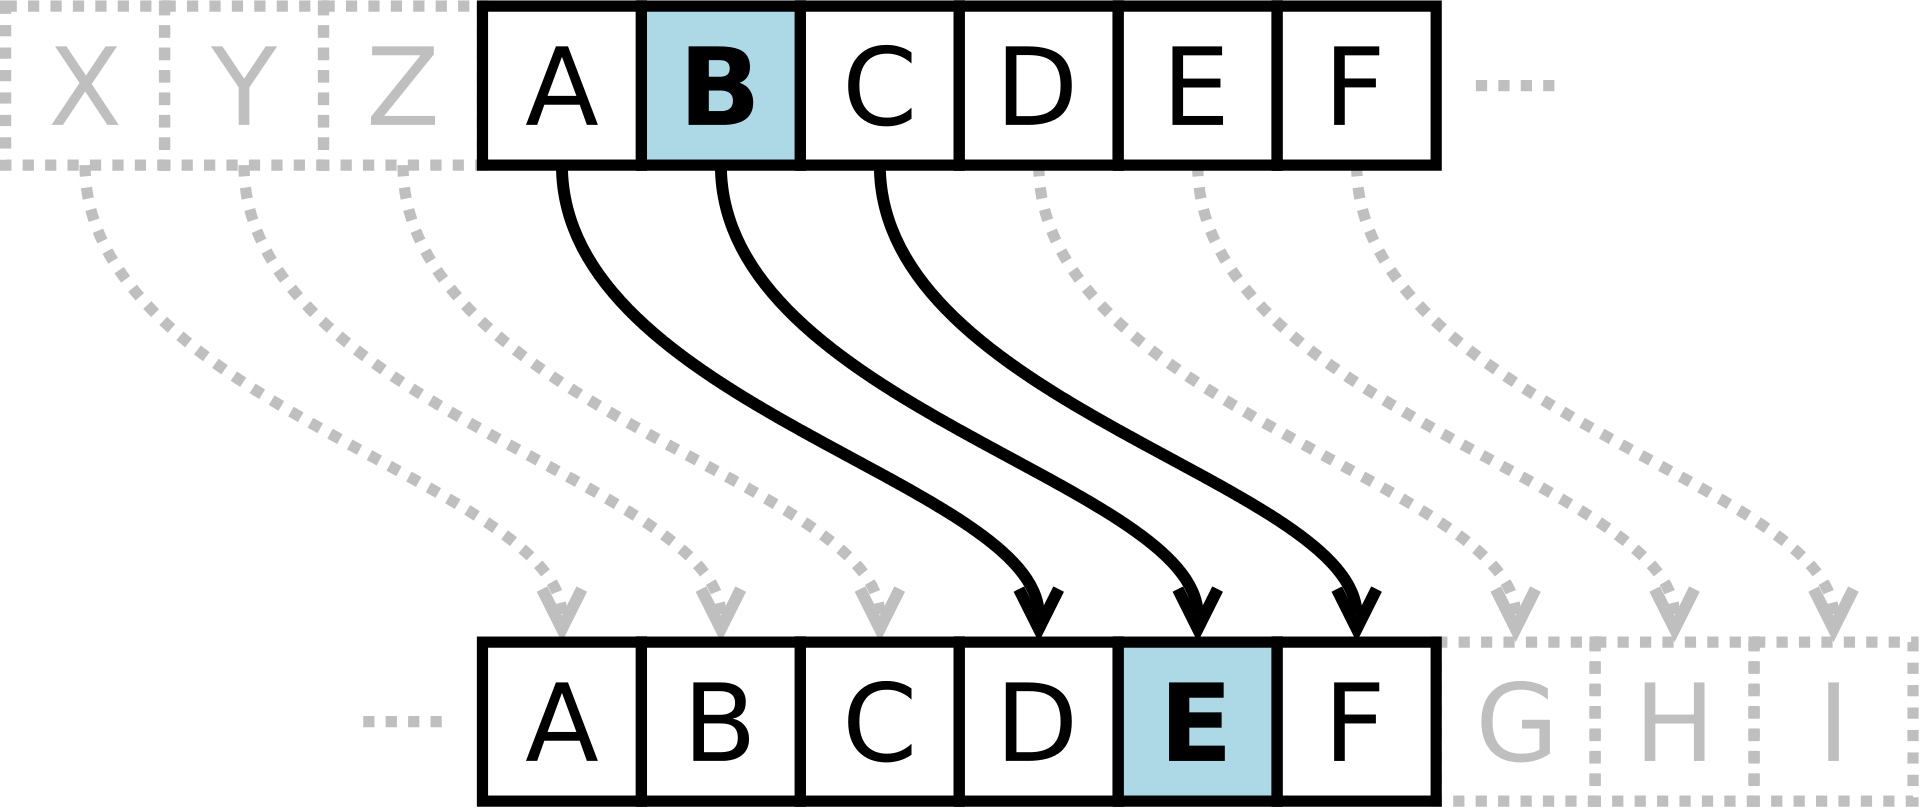
\includegraphics[width=0.5\textwidth]{pic/2.1.png}
    \caption{«шифр Цезаря»}
    \label{fig:cez}
\end{figure}

Основоположником «шифра» в России является Иван Грозный, создавший «циферное отделение». В свою очередь, в 1702 году Пётр I 
учредил посольскую канцелярию, которая придумывала шифры и занималась расшифровкой текстов от иностранных послов. Ниже на рисунке ~\ref{fig:petr}, представлен пример Шифра Петра I.

\begin{figure}[h]
    \centering
    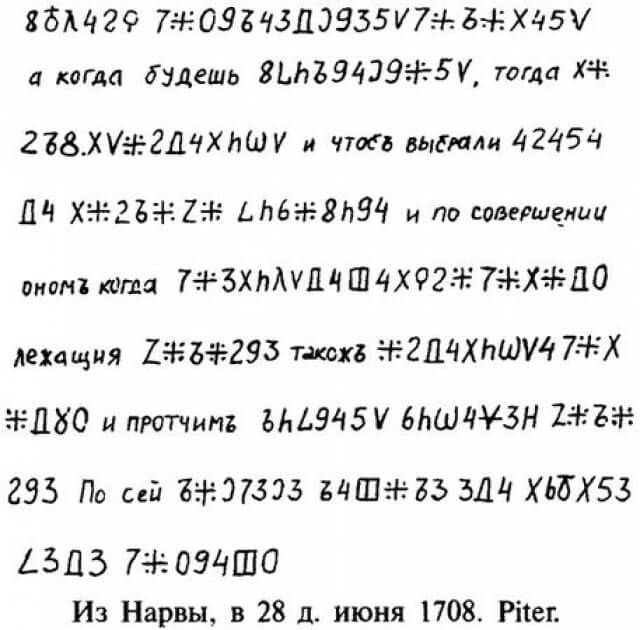
\includegraphics[width=0.4\textwidth]{pic/2.2.jpg}
    \caption{«шифр Петра I»}
    \label{fig:petr}
\end{figure}

В следующем этапе развития методов защиты информации произошел значительный прорыв с появлением и широким распространением 
технических средств защиты, включая роторные машины. Одним из первых примеров таких машин была Enigma, созданная немецкими 
изобретателями Эдвардом Хеберном и Артуром Кирхом в 1917 году. Роторные системы были важным средством защиты конфиденциальной 
информации в то время, например во время Второй мировой войны такие системы, как Enigma (Германия), Sigaba (США), Турех 
(Великобритания), Red, Orange и Purple2 (Япония) были широко использованы. Однако только с развитием компьютеров в начале 
40"=х годов стали возможны успешные крипто"=атаки на роторные системы. В то же время, методы защиты от технических утечек 
информации совершенствовались, что способствовало развитию технической разведки государственными и коммерческими 
организациями.

С появлением первых компьютеров вместе с их развитием и интеграцией в общество, кодировка с использованием блочных шифров стала более распространенной и надежной альтернативой роторным системам из"=за их высокой скорости обработки и передачи 
информации. Прорыв в области информационной безопасности случился в 1970"=е годы с появлением первых вирусов и хакеров, что 
привело к необходимости разработки новых методов защиты, таких как антивирусное программное обеспечение, межсетевые экраны и 
системы обнаружения вторжений.

В 1977 году был принят стандарт шифрования DES в США, разработанный компанией IBM, который послужил основой для многих других 
моделей криптосистем по всему миру. С развитием интернета в 1990"=е годы информационная безопасность стала более актуальной 
проблемой из"=за появления новых угроз, таких как фишинг, спам и DDoS"=атаки. Для противодействия этим угрозам были разработаны 
новые методы защиты, такие как шифрование данных, аутентификация пользователей и защита от DDoS\cite{sforum}.

На современном этапе развития общества информация выступает как форма собственности, и следовательно, имеет определенную 
ценность. Чтобы подчеркнуть роль информации в обществе, говорят об «информационном обществе», в отличие от предыдущей фазы 
развития общества "---  «индустриальном обществе». Начиная с 90"=х гг. ХХ в. исследованиями в области информационной безопасности 
активно занимаются российские ученые. В.А. Герасименко разработал системно"=концептуальный подход к обеспечению информационной 
безопасности автоматизированных систем обработки данных. А.А. Грушо и Е.Е. Тимонина представили доказательный подход к 
проблеме гарантированности защиты информации в компьютерной системе. А.А. Грушо в сферу исследований были введены новые виды 
скрытых каналов утечки информации, основывающихся на использовании статистических характеристик работы системы. С.П. 
Расторгуев и А.Ю. Щербаков разработали теорию разрушающих программных воздействий. А.Ю. Щербаковым также была разработана 
субъектно"=объектная модель системы, на базе которой сформированы понятия информационных потоков и доступов в компьютерной 
системе. 

В настоящее время теория информационной безопасности продолжает развиваться. Появляются новые угрозы и вызовы, связанные с 
развитием информационных технологий. Это требует разработки новых методов и средств защиты информации\cite{urfu}.

\newpage
\subsection{Необходимость защиты информации.}
Бурное развитие средств вычислительной техники открыло перед человечеством непревзойденные возможности для автоматизации 
умственного труда, приведя к появлению многочисленных автоматизированных информационных и управляющих систем, а также к 
зарождению совершенно новых информационных технологий. Некоторые психологи считают, что человек разумный постепенно 
превращается в человека информационного.

Доступность вычислительной техники, особенно персональных компьютеров, привела к распространению компьютерной грамотности в 
широких кругах населения, что, естественно, привело к увеличению числа попыток незаконного вторжения в работу государственных 
и коммерческих автоматизированных систем "--- как с злым умыслом, так и чисто <<из спортивного интереса>>. К сожалению, многие из 
таких попыток приводят к успеху и наносят значительный ущерб всем заинтересованным сторонам информационных отношений.

При анализе проблем, связанных с информационной безопасностью, следует учитывать специфику данной сферы. Он 
является составной частью информационных технологий, сферы, которая развивается с поразительной скоростью. Тут важны не 
только отдельные решения (законы, учебные курсы, программно"=технические изделия), соответствующие современному уровню, но и 
механизмы создания новых решений, позволяющие им следовать темпу технического прогресса. К сожалению, существующая на 
сегодняшний день технология программирования не обеспечивает создание безупречных программ, что затрудняет быстрое развитие 
средств обеспечения информационной безопасности. Необходимо создавать надежные системы (информационной безопасности) с 
использованием ненадежных компонентов (программ). В принципе, это возможно, но требует соблюдения определенных архитектурных 
принципов и контроля за уровнем защищенности на протяжении всего жизненного цикла программы.

Увеличение числа атак "--- не самое страшное. Хуже то, что непрерывно обнаруживаются новые уязвимые места в программном 
обеспечении (связываемое с ограничениями современной технологии программирования) и, как следствие, возникают новые виды атак.

В этих условиях системы информационной безопасности должны быть способны противостоять различным атакам, как внешним, так и 
внутренним, автоматизированным и скоординированным. Иногда атаки длительны всего лишь доли секунды; порой поиск уязвимостей 
проводится медленно, растягивается на часы, так что подозрительная деятельность почти незаметна. Целью злоумышленников может 
быть нарушение всех аспектов информационной безопасности "---  доступности, целостности или конфиденциальности\cite{biblio}.

\section{Основные составляющие защиты информации.}
\subsection{Виды угроз и способы защиты.}
Появление новых информационных технологий и развитие мощных компьютерных систем хранения и обработки информации повысили уровни защиты информации и вызвали 
необходимость в том, чтобы эффективность защиты информации росла вместе со сложностью архитектуры хранения данных. Так постепенно защита экономической информации 
становится обязательной: разрабатываются всевозможные документы по защите информации; формируются рекомендации по защите информации; даже проводится федеральный закон 
о защите информации. В правовых основах защиты информации можно выделить 4 основных уровня:
\begin{itemize}
    \item \textbf{Первый уровень.} Состоит из из международных договоров о защите информации и государственной тайны;
    \item \textbf{Второй уровень.} Здесь находятся подзаконные акты "--- указы президента, постановления Правительства и т.д;
    \item \textbf{Третий уровень.} К данному уровню обеспечения правовой защиты информации относятся ГОСТы безопасности информационных технологий, а также обеспечения безопасности информационных систем.
    Также на третьем уровне безопасности информационных технологий присутствуют руководящие документы, нормы информационной безопасности и классификаторы, разрабатывающиеся 
    государственными органами;
    \item \textbf{Четвёртый уровень.} Образуют локальные нормативные акты, инструкции и положения по комплексной правовой защите.\cite{def_inf}
\end{itemize}
Виды угроз и атак также делят на несколько категорий. Среди категорий выделяют:
\begin{itemize}
    \item Перехват электронных излучений. Проблема решается обеспечением защиты информации, передаваемой по радиоканалам связи и обмена данными 
    информационной системы;
    \item Применение подслушивающих устройств;
    \item Использование недостатков языков программирования с целью маскирования под запросы системы;
    \item Злоумышленный вывод из строя технологий и механизмов;
    \item Информационные утечки.
\end{itemize}

У всех вышеперечисленных угроз одна общая цель, а именно "--- призвать утечку информации юридического лица, кампании.

\newpage
\subsection{Утечки информации и их последствия.}
С увеличением масштабов распространения и использования ЭВМ и информационных сетей усиливается роль различных факторов, вызывающих утечку, 
разглашение и несанкционированный доступ к информации. К ним относятся:
\begin{itemize}
    \item Ошибки пользователей и персонала;
    \item Технические сбои;
    \item Природный фактор (природные явления, аварии).
\end{itemize}
В наши дни количество зарегистрированных случаев утечек информации с каждым годом только растёт. Утечка происходит как и намеренно, с целью получения
материальной выгоды, так и случайно, например, из"=за несоблюдения персоналом правил информационной безопасности. Именно на этой основе все утечки фирмы или кампании
делятся на \textbf{умышленные} и \textbf{неумышленные.} К сожалению, в силу халатности и неправомерных действий сотрудников, нередки случаи утечки информации или целых
баз данных.

\subsection{Принципы информационной безопасности.}
Существует 3 основных принципа информационной безопасности, которые основываются на свойствах информации: конфиденциальность, целостность и доступность информации.

\textbf{Принцип конфиденциальности} постулирует необходимость обеспечения возможности получения передаваемой информации только адресатом. Из этого вытекает, что передаваемая информация
не должна быть получена \textbf{и считана} третьими лицами, в частности злоумышленниками.

\textbf{Принцип целостности} заключается в корректности и неизменности передаваемой информации. За время передачи информации получателю, информация должна оставаться полной и актуальной.
Помимо этого, информация должна сохранять первозданный вид, несмотря на внешние искажения.

\textbf{Принцип доступности} говорит о том, что доступ к передаваемой информации должны иметь только легитимные пользователи, то есть только те пользователи, которым изначально
передавалась информация.

Осуществление и выполнение подобных принципов достигается различными методами защиты от внеших угроз, о которых будет сказано ниже.


\newpage
\subsection{Классификация средств защиты информации. Методы защиты данных. Шифрование.}
В своей основе, средства защиты информации классифицируются на \textbf{формальные} и \textbf{неформальные.} Формальные средства защиты информации подразумевают исполнение процедур по защите 
без вмешательства человека, в то время как неформальные "--- полностью основанны на действиях человека.

Среди основных методов защиты информации выделяют:
\begin{itemize}
    \item \textbf{Криптографические} "--- защита данных, передаваемых по глобальной или корпоративной сети. Включает в себя различные типы шифрования, в частности с использованием специальных аппаратов
    и программ;
    \item \textbf{Физические} "--- средства и механизмы, работающие вне зависимости от информационных систем;
    \item \textbf{Программные} "--- защита передаваемой информации посредством специального ПО, настроенного под конкретную сеть и конкретные задачи.
\end{itemize}

В своей сути у большинства метода заложен различный метод \textbf{шифрования.} Шифрование "--- это процесс преобразования информации путём исполнения конкретного алгоритма с целью сохранения конфиденциальности
данной информации. Существует также процесс, обратный шифрованию "--- \textbf{дешифрование.} Преобразование производится согласно выбранному алгоритму шифрования 
и, отталкиваясь от этого, выполняется определённая процедура.

\textbf{Криптография} предлагает множество вариантов шифрования, и, соответственно, дешифрования, однако к классическим методам принято относить \textbf{симметричное шифрование.} Это тип шифрования, в котором и для шифрования, и для дешифрования,
используется единый криптографический ключ. Основным условием симметричного шифрования является факт того, что отправитель и получатель информации заранее знают о 
методе шифрования и заранее имеют на руках криптографический ключ, который необходимо держать в секрете с обеих сторон. Однако у симметричного шифрования существует ряд недостатков: наличие ключа как у отправителя, так и у получателя.
Из этого следует, что изначально сам ключ должен быть передан безопасным путём. Решает эти проблемы не менее популярное \textbf{ассиметричное шифрование,} при котором для шифрования и для шифрования используются, соответственно, два разных ключа.
Так, ключ для дешифрования генерируется у получателя, которому достаточно знать только метод шифрования.\cite{shifr}






\section{Профессиональное развитие и карьерные перспективы.}
\subsection{Кто такой специалист по защите информации сейчас.}
\textbf{Специалист по защите информации} "---  это высококвалифицированный специалист, который ответственен за защиту конфиденциальных 
данных, информационных систем и сетей от утечек, кражи и других видов злоупотреблений. С увеличением объема и ценности 
информации, хранимой и передаваемой в цифровом формате, растет и важность профессионального защитника информации.

Основные обязанности специалиста по защите информации включают разработку и внедрение мер безопасности информационных систем, 
анализ уязвимостей, прогнозирование и предотвращение кибератак, обучение сотрудников правилам безопасности. Также в их 
компетенции находится расследование инцидентов безопасности, разработка политики безопасности и соблюдение соответствующих 
законов и стандартов.
Но есть и более узкие специальности уже внутри сферы:
\begin{itemize}
    \item \textbf{Пентестеры} "---  так называемые «белые» или «этичные» хакеры. Они не взламывают ресурсы бизнеса незаконно. Вместо 
    этого они работают на компании и ищут уязвимости, которые потом исправляют разработчики. Бывает, такие люди трудятся на 
    окладе, или участвуют в программах Bug Bounty "---  когда бизнес просит проверить их защиту, обещая за найденные баги премию.
    \item \textbf{Специалисты по разработке} "--- такие специалисты участвуют создании приложений и программ. Проще говоря, 
    изучают архитектуру и готовый код и подсказывают, что здесь может быть ошибка или «форточка» для взлома. Банальный пример 
    "---  оставить в форме ввода сайта возможность отправить SQL-инъекцию.
    \item \textbf{Специалисты по сетям} "---  они ищут возможные потенциальные и известные уязвимости в аппаратных и сетевых 
    комплексах. Проще говоря, знают, как с помощью Windows, Linux или других систем злоумышленник может попасть в ваш 
    компьютер и установить нужное ПО. Могут как найти возможность взлома, так и создать систему, в которую будет сложно 
    попасть.
\end{itemize}
Есть ещё один вариант деления специалистов:
\begin{itemize}
    \item Отвечающие за взлом, к примеру, сети или программы. Иначе называется этичный хакинг "---  специализация на обнаружении ошибок и уязвимостей.
    \item Отвечающие за создание и поддержку систем защиты. Этот вариант работодатели подразумевают, когда ищут специалиста по защите информации\cite{habr}.
    
\end{itemize}

Для успешной работы специалист по защите информации должен обладать знаниями в области информационных технологий, 
криптографии, сетевой безопасности, законодательства о защите данных. Он также должен иметь навыки аналитического мышления, 
умение принимать быстрые и правильные решения в экстренных ситуациях, уметь анализировать риски информационной безопасности и 
предлагать эффективные меры по их минимизации, а также быть готовым к постоянному обучению и развитию.

В современном мире спрос на специалистов по защите информации растет, так как компании и организации всё чаще сталкиваются с 
киберугрозами, взломами и другими атаками на информационную инфраструктуру. Поэтому специалисты по защите информации являются 
востребованными специалистами на рынке труда и обладают хорошими перспективами карьерного роста.
Из-за неустоявшихся терминов есть небольшая путаница и в названиях вакансий — компании ищут специалистов по информационной 
безопасности, администраторов защиты, инженеров безопасности компьютерных сетей и другие названия, подразумевая одного и того 
же специалиста.
\newpage
\subsection{Типы <<хакеров>>: черные, белые, серые.}
Если вы смотрите новости и следите за технологиями, вы знаете, кто такие хакеры. Однако не все знают, что хакеры делятся на категории, называемые Черные шляпы, Белые шляпы и Серые шляпы. Эти термины берут свое начало в американских вестернах, где главные герои носили белые или светлые шляпы, а отрицательные персонажи "---  черные шляпы.
По сути, тип хакера определяется его мотивацией и тем, нарушает ли он закон.

\textbf{Кто же такие <<Чёрные шляпы>>?}
«Чёрные шляпы» "---  это хакеры, которые используют свои навыки для незаконного проникновения в компьютерные системы и кражи данных. Они могут быть как начинающими дилетантами, так и опытными профессионалами, работающими на крупные преступные организации.

Хакерство может действовать как крупный бизнес, масштабы которого позволяют легко распространять вредоносные программы. У организаций есть партнёры, торговые посредники, поставщики и совладельцы, которые покупают и продают лицензии на вредоносное ПО другим преступным организациям для использования в новых регионах и на новых рынках.

Взломы, осуществляемые <<Чёрными шляпами>>, являются глобальной проблемой, которую крайне сложно решить. Работа 
правоохранительных органов осложняется тем, что хакеры оставляют мало улик, используют компьютеры ничего не подозревающих 
жертв и действуют в нескольких юрисдикциях. Иногда властям удаётся закрыть хакерский сайт в одной стране, однако эти же 
действия могут выполняться в другом месте, что позволяет преступной группе продолжать работу.

\textbf{В противоположность <<чёрным>> \ есть <<белые>> \  хакеры.} <<Белые шляпы>> "---  это специалисты по безопасности, которые выявляют недостатки в защите компьютерных систем и сетей с целью их устранения. Они работают на компании или являются независимыми 
подрядчиками. Их деятельность помогает предотвратить несанкционированный доступ к данным и снизить вероятность кибератак.
<<Чёрные шляпы>> получают незаконный доступ к системам со злыми намерениями и часто с целью личного обогащения. В отличие от 
них, <<Белые>> сотрудничают с компаниями и помогают им устранять слабые места в их системах, чтобы гарантировать 
безопасность данных.

\textbf{Но также существует что-то среднее между <<чёрными>> и <<белыми>>,} так называемые <<Серые шляпы>> "---  это хакеры, которые ищут 
уязвимости в системах без разрешения или ведома владельца. Они могут сообщать о найденных уязвимостях владельцу за небольшую 
плату.

Некоторые Серые шляпы считают, что их действия приносят пользу компаниям, но владельцы компаний редко ценят 
несанкционированные вторжения. Часто реальный мотив Серых шляп "---  продемонстрировать навыки и добиться известности.

Серые шляпы иногда нарушают законы и стандарты этики, но не имеют злого умысла, характерного для <<Чёрных шляп>>. В отличие от 
Белых шляп, они не связаны этическими правилами взлома или трудовым договором. Если организация не обращает внимания на их 
действия, они могут использовать обнаруженные уязвимости самостоятельно или рассказать о них другим хакерам\cite{kaspersky}.


\newpage
\subsection{Плюсы и минусы работы в области защиты информации.}
Плюсы:
\begin{enumerate}
    \item На специалистов по защите информации сейчас высокий спрос, с каждым годом количество различных угроз и кибератак 
    стремительно увеличивается, что делает специалистов этой сферы ещё более востребованными.
    \item Стремительные изменения в сфере информационных технологий позволяют специалистам получать бесценный опыт и 
    постоянное профессиональное развитие, постоянно обучаясь и повышая свою квалификацию.
    \item Благодаря высокой востребованности данной сферы, специалисты получают достаточно высокую заработную плату.
\end{enumerate}
 
Минусы:
\begin{enumerate}
    \item Работа под постоянным давлением и стрессом "---  нужно мгновенно реагировать на угрозы кибербезопасности и защищать 
    информацию от внешних угроз.
    \item Большая ответственность за сохранность и конфиденциальность большого количества информации.
    \item Высокие требования к профессиональным навыкам: работа в области защиты информации требует наличия 
    специализированных знаний и опыта, которые не всегда могут быть легко достигнуты.
\end{enumerate}
\section{Роль и обязанности специалиста по защите информации.}
\subsection{Защита от внешних угроз.}
    Одной из обязанностей специалиста в данной сфере является защита передаваемой информации от потенциальной фальсификации. Вопросами, связанными с конфиденциальностью и 
    сохранностью передаваемой информации, занимается
    \textbf{криптография.} Это раздел математики, ассоциирующийся с кодированием данных, однако это не совсем так.
    Помимо этого, криптография также охватывает вопросы, связанные с подменностью цифровых данных, а именно: проверка достоверности
    цифровых данных, верификация этих данных.

    Примером такого механизма защиты данных является \textbf{электронная цифровая подпись(ЭЦП)}. ЭЦП "--- реквизит электронного документа, предназначенный для 
    защиты данного документа от подделки, полученный в результате криптографического преобразования
    информации с помощью закрытого ключа электронной цифровой подписи. ЭЦП позволяет идентифицировать владельца сертификата
    ключа подписи. Помимо этого, ЭЦП является необходимым атрибутом любого электронного документа и делается в виде специально
    закодированной строки при помощи новейших технологий.  

    Электронная цифровая подпись состоит из 3"=х основных элементов:

    \begin{enumerate}
        \item Сертификат;
        \item Открытый ключ;
        \item Закрытый ключ.
    \end{enumerate}

    В сертификате находится краткая информация о владельце, а ключи состоят из закодированных символов. 

    \begin{figure}[H]
        \centering
        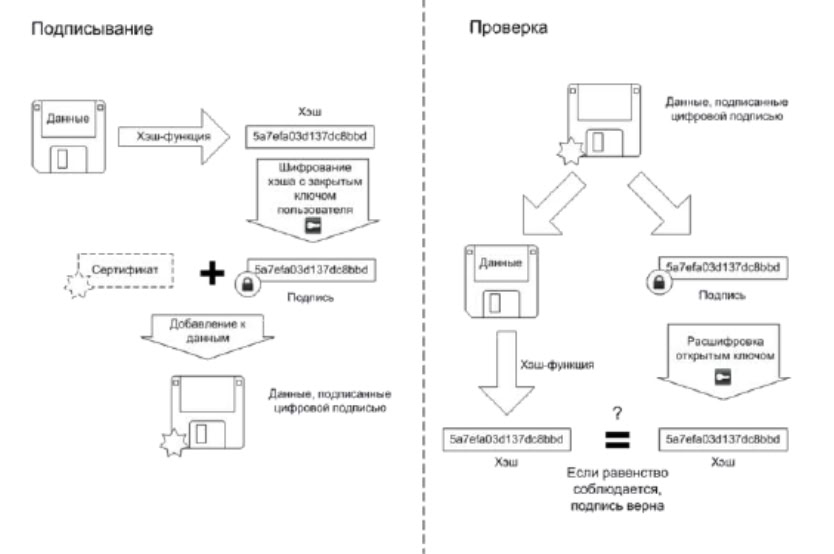
\includegraphics[height = 11cm, width = 14cm]{pic/legit_doc.png}
        \caption{Пример работы ЭЦП}
    \end{figure}

    ЭЦП была произведена для исполнения сделок различного рода между юридическими лицами в интерактивном режиме,
    а также для обмена важной информацией, которая нуждается в конфиденциальности. За счёт криптографического преобразования,
    документ имеет ряд символов, которые возникают посредством работы ПО, создающего электронную подпись. Таким образом, данный документ
    может открыть только тот пользователь, которому он был отправлен.

    Исходя из вышесказанного, ЭЦП даёт гарантию, что авторское право документа не подлежит фальсификации.\cite{crypto}

\newpage
\subsection{Мониторинг систем информационной безопасности.}
    Безопасность информационных систем основывается на защите систем от уязвимостей, которые в свою очередь могут возникать из"=за
    ошибок в конфигурации компонентов информационной системы. \textbf{Мониторинг информационной безопасности} представляет собой процесс систематического 
    наблюдения, анализа и контроля за состоянием безопасности информационных систем и данных. Он осуществляется с помощью специализированных программных и 
    аппаратных средств, которые позволяют выявлять, предотвращать и реагировать на возможные угрозы, нарушения и аномалии в информационной среде организации.
    Основная цель мониторинга "--- обнаружение ошибок конфигурации и инцидентов в режиме реального времени, чтобы минимизировать ущерб для конкретной компании.
    Помимо этого, мониторинг информационной безопасности позволяет предотвратить возможные атаки.

    \begin{figure}[H]
        \centering
        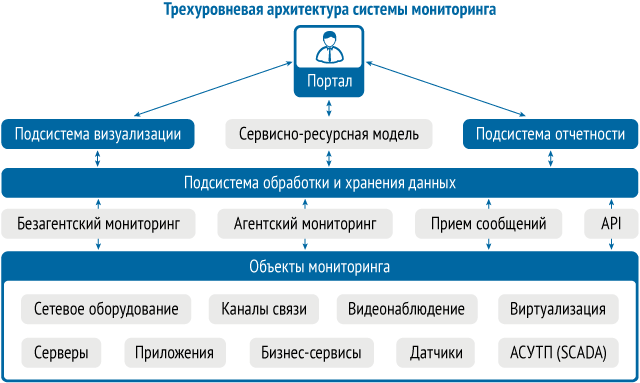
\includegraphics[width = 14cm]{pic/monitoring.png}
        \caption{Дерево мониторинга систем}        
    \end{figure}

    \newpage
    Мониторинг систем информационной безопасности является комплексным процессом, который выполняется в несколько этапов:

    \begin{enumerate}
        \item \textbf{Сбор данных и логов.}
            Мониторинг начинается со сбора данных из различных информационных систем. Эти данные представляют основу для анализа безопасности;
        \item \textbf{Анализ данных.}
            Собранные данные проходят через определенные алгоритмы анализа данных с целью выявления различных угроз или аномалий;
        \item \textbf{Обнаружение инцидентов.}
            На данном этапе мониторинг позволяет выявить различные угрозы, что позволяет оперативно среагировать на них;
        \item \textbf{Реагирование на инциденты.}
            Команда специалистов по обеспечению безопасности должна иметь определенный план реагирования для различных сценариев. Мониторинг
            в свою очередь помогает минимизировать ущерб от атак;
        \item \textbf{Отчет и анализ производительности.}
            Мониторинг систем информационной безопасности также включает в себя анализ эффективности применяемых мер и создание отчётов о безопасности.\cite{monitoring}
    \end{enumerate}

    Однако несмотря на уровень профессионализма специалистов, всё равно периодически происходят атаки на информационные системы. В этом случае, специалист 
    должен провести процедуру \textbf{восстановления после атаки.} 

\newpage
\subsection{Восстановление после атак. Резервное копирование информации.}
    \textbf{Кибератака} (или атака на информационную систему) "--- комплекс действий, нацеленный на нарушение доступности и конфиденциальности информации.
    Успешная кибератака может привести к существенной утечке данных и важной информации компании.
    В случае, если атака всё же произошла, специалисту по защите информационной безопасности необходимо разработать сценарий действий и согласовать его 
    с остальными сотрудниками. В зависимости от "силы" проведённой атаки может потребоваться значительное количество средств и времени на восстановление.

    Рассмотрим один из самых популярных методов восстановления информации "--- восстановление через \textbf{резервное копирование}. Само резервное копирование 
    может проводиться с помощью физического носителя (например, жесткий диск), облачного хранилища, или с помощью гибридного метода, подразумевающего использование
    как и физического носителя, так и облачного хранилища. В зависимости от ресурсов кампании и согласованного сценария, применяется один из этих методов восстановления.
    Резервное копирование может осуществляться различными способами. В этой статье будут рассмотренны основные и самые популярные.\cite{main_methods}

    \textbf{Полное резервное копирование} "--- копирование абсолютно всей информации. С его помощью можно восстановить всю информацию в любой момент времени. Основным минусом
    этого метода является требуемый объём памяти. Помимо этого, восстановление данных этим методом предполагает полную замену, что может занять значительное время.

    \textbf{Инкрементальное резервное копирование} "--- процесс копирования, при котором старые (т.е. уже сохраненные) данные остаются без изменений, а новые данные,в том числе и утерянные, 
    восстанавливаются. При использовании данного метода, создаются несколько копий данных, а именно нулевая и инкрементные копии, где нулевая копия является полной.

    \textbf{Дифференциальное резервное копирование} "--- данный процесс использует разницу между двумя версиями данных. Первоначально создаётся полная копия, затем копируются изменения.

    В зависимости от выбранного метода восстановления, определяются ресурсы и время, необходимые для полного восстановления.


\newpage
\subsection{Обучение сотрудников правилам безопасности.}

    В период восстановления после атак активно продумывается каждый этап восстановления, в том числе и снижение будущих
    потенциальных рисков подобных угроз. Одним из самых важных аспектов восстановления является обучение сотрудников правилам безопасности.
    
    В зависимости от масштаба, причины и метода произведённой атаки, специалист обязан провести обучение с целью подготовить сотрудников фирмы 
    к подобным атакам. Его задача - предотвратить использование определённого ПО сотрудниками в случае, если причиной атаки стало именно оно,
    подготовить и согласовать сценарий действий в случае, если подобная атака повторится ещё раз. Помимо этого, специалист должен выработать
    определённые правила конфиденциальности информации в фирме на время уязвимости после произведённой атаки.






\conclusion
Специалист по защите информации "--- высококвалифицированный сотрудник, который необходим каждой фирме,
которая заботится о безопасности своих данных. В ходе работы мы выяснили, что такое защита информации и мониторинг систем информационной безопасности, каким атакам
может подвергнуться информационная система и какие существуют методы борьбы с действиями злоумышленников. Помимо этого,
удалось рассмотреть основные задачи специалиста по защите информации, какими навыками должен обладать специалист в данной сфере,
а также его обязанности в фирме или кампании.
% Библиографический список, составленный вручную, без использования BibTeX
%
% \begin{thebibliography}{99}
%   \bibitem{Ione} Источник 1.
%   \bibitem{Itwo} Источник 2
% \end{thebibliography}

% Отобразить все источники. Даже те, на которые нет ссылок.
% \nocite{*}

% Меняем inputencoding на лету, чтобы работать с библиографией в кодировке
% `cp1251', в то время как остальной документ находится в кодировке `utf8'
% Credit: Никита Рыданов
\inputencoding{cp1251}
\bibliographystyle{gost780uv}
\bibliography{thesis}
\inputencoding{utf8}

% При использовании biblatex вместо bibtex
% \printbibliography

% Окончание основного документа и начало приложений Каждая последующая секция
% документа будет являться приложением
\appendix

\end{document}
